% fancytikzposter.tex, version 2.1
% Original template created by Elena Botoeva [botoeva@inf.unibz.it], June 2012
%
% This file is distributed under the Creative Commons Attribution-NonCommercial 2.0
% Generic (CC BY-NC 2.0) license
% http://creativecommons.org/licenses/by-nc/2.0/


\documentclass[20pt]{a0poster}

\usepackage{fancytikzposter}
\usetemplate{2}

\usepackage[utf8]{inputenc}
\usepackage[margin=\margin cm, paperwidth=84.1cm, paperheight=118.9cm]{geometry}

\usepackage{fancyvrb}

%% changing the fonts
\usepackage{cmbright}
%\usepackage[default]{cantarell}
%\usepackage{avant}
%\usepackage[math]{iwona}
\usepackage[math]{kurier}
\usepackage[T1]{fontenc}
\usepackage{transparent}

%% add your packages here
\usepackage{hyperref}
\usepackage[shortlabels]{enumitem}

% http://www.latex-community.org/forum/viewtopic.php?f=44&t=7894
\setitemize{labelindent=1em,labelsep=0.5cm,leftmargin=*}
\renewcommand{\labelitemi}{$\bullet$}
\renewcommand{\labelitemii}{$\cdot$}
\renewcommand{\labelitemiii}{$\diamond$}
\renewcommand{\labelitemiv}{$\ast$}
\newcommand{\bkpspace}{\kern-2.8em}

%\renewcommand*\rmdefault{iwona}
\usepackage{helvet}
\renewcommand{\familydefault}{\sfdefault}
\newcommand*\circled[1]{\tikz[baseline=(char.base)]{
            \node[shape=circle,draw=black!80,line width=1mm,inner sep=2pt] (char) {#1\quad};}\,}
\newcommand*{\mystrut}{\rule[-.15\baselineskip]{0pt}{0.8\baselineskip}}
\newcommand*\rectangled[1]{\tikz[baseline=(char.base)]{
            \node[shape=rectangle,draw=black!80,line width=1mm,inner sep=5pt, rounded corners=8pt,fill=white] (char) {\mystrut #1};}}

% \sethlcolor{white}
% \renewcommand*\rectangled[1]{\hl{#1}}

\usepackage{ulem}

\usepackage{graphicx}
\usepackage{epstopdf}
\usepackage{pst-barcode}

% \definecolor{light-gray}{gray}{0.0}
\definecolor{light-grey}{HTML}{888888}
\definecolor{light-light-grey}{HTML}{EEEEEE}

% ldl
%\definecolor{light-red}{HTML}{d0e3d0}%{E3DEDE}
%\definecolor{dark-red}{HTML}{004500}%{FF7F00}

% ildl
\definecolor{ecocloud-blue}{RGB}{63,63,63}%{HTML}{0a4d6b}%{1075bb}
\definecolor{light-red}{HTML}{eaeaea}%{E3DEDE}
\definecolor{dark-red}{RGB}{63,63,63}%{5b5c5b}%{FF7F00}
\definecolor{dark-red-title}{RGB}{100,100,100}%{5b5c5b}%{FF7F00}

% \definecolor{light-red}{HTML}{ebeceb}%{E3DEDE}
% miniboxing
% \definecolor{light-gray}{HTML}{E3DEDE}
%  \definecolor{darkred}{RGB}{160,0,0}

\setblockfillcolor{light-red}
\setblocktitletextcolor{dark-red}
\setinnerblocktitlefillcolor{dark-red-title}

\renewcommand\BackgroundPicture{
  % \node[anchor=south west,inner sep=0] at (0,0) {\includegraphics{};
  %   \addlogo[south west]{(0.0,0.0)}{90mm}{ldl-frog.pdf}
  % }
  \put(0,0){\parbox[b][\paperheight]{\paperwidth}{\vspace{40mm}\left\kern44mm
\includegraphics[width=250,keepaspectratio]{ldl-frog.pdf}\vfill}}
}

\newcommand\ttt[1]{\texttt{#1}}
\newcommand\tth[1]{\rectangled{\code{}{#1}}}
\newcommand\code[2]{\textcolor{white}{\texttt{\frenchspacing{}#1}}\texttt{\frenchspacing{}#2}}
\newcommand\comment[1]{\textcolor{light-grey}{\texttt{\frenchspacing{}#1}}}
\newcommand\ropt[1]{\rectangled{\kern0.2em #1 \kern0.0em}}
\newcommand\roptn[1]{#1}
\newcommand\startOfBox{\Large\vspace{0.0em}}
\newcommand\separator{\vspace{0.8em}}
\newcommand\codebox[2]{\vspace{-0.2em}\innerblock{#1}{#2}\vspace{-0.8em}}
\newcommand\codeboxx[2]{\vspace{-0.1em}\innerblockplain{#2}\vspace{-0.8em}}

\newenvironment{pitemize}{
  \vspace{0.2em}
  \begin{itemize}
  \setlength{\itemsep}{0.15em}
  \setlength{\parskip}{0.2pt}
  \setlength{\parsep}{0.2pt}
}{
  \end{itemize}
  \vspace{-0.1em}
}

% Set underline thickness
% http://latex-community.org/forum/viewtopic.php?f=44&t=18362
\usepackage{soul}
\setul{4pt}{4pt}

% \usepackage{lmodern}
% \renewcommand{\ttdefault}{pcr}

\title{
\raggedright
  \vspace{-3mm}\LARGE{\textbf{Automating Ad hoc Data Representation Transformations (OOPSLA'15)}\bkpspace}\vspace{-2mm}
}
\author{
  Vlad Ureche$^\dagger$ \kern1em Aggelos Biboudis$^*$ \kern1em Yannis Smaragdakis$^*$ \kern1em Martin Odersky$^\dagger$\\
  École polytechnique fédérale de Lausanne, Switzerland$^\dagger$ \kern1em University of Athens$^*$ \\
  \texttt{\frenchspacing{}\{first.last\}@epfl.ch$^\dagger$ \frenchspacing{}biboudis@di.uoa.gr \frenchspacing{}smaragd@di.uoa.gr \; \texttt{\frenchspacing{}scala-ldl.org}}
  \vspace{-17mm}
}

\usepackage{soul}
\sethlcolor{light-light-grey}

\begin{document}

%%%%% ---------- the background picture ---------- %%%%%
%% to change it modify the macro \BackgroundPicture
\ClearShipoutPicture
\AddToShipoutPicture{\BackgroundPicture}

\noindent % to have the picture right in the center
\begin{tikzpicture}
  \initializesizeandshifts
  % \setxshift{15}
  % \setyshift{2}

  %% the title block, #1 - shift, the default value is (0,0), #2 - width, #3 - scale
  %% the alias of the title block is `title', so we can refer to its boundaries later
  \ifthenelse{\equal{\template}{1}}{
    \titleblock[(0,0)]{47}{1}
  }{
    \titleblock[(20, -0.5)]{47}{1.5}
  }

  %% a logo can be added to the title block
  %% #1 - anchor relative to the title block, #2 - shift, #3 - width, #3 - file name
%   \addlogo[south west]{(-2,0.0)}{90mm}{ldl-frog.pdf}

  \blocknode%
    {\circled{1} Data Representation Problem}%
    {\startOfBox
        In high-level languages, such as Scala, developers write their data structures using generic components from the library:

        \separator

        % For example, the source code: \\[-0.5em]

%         \innerblockplain{
        \codebox{Library Class}{
          \code{}{class Vector[+A] extends Sequence[A] with ... \{  } \\ %\;\comment{// value 5 has type Int and} \\
          \code{..}{...} \\   %\;\comment{// Int is a subtype of Any}
          \code{}{\}}    %\;\comment{// Int is a subtype of Any}
        }

        Library components are freely mixed with custom data structures. For example, with objects storing sensor readings:

        \separator

        \codebox{Source Code}{
          \code{}{case class SensorReading(timestamp: Int,} \\
          \code{.........................}{sensor: Int,} \\
          \code{.........................}{value: Double)}
        }

        Programmers appreciate the ability to mix data structures, as it increases productivity. Yet, without realizing, they give up performance, as the mixed data structures have suboptimal memory rep\-re\-sen\-ta\-tions.

        \separator

        In our example, traversing a \ropt{\texttt{Vector[SensorReading]}} object requires a pointer dereference for each element:

        \separator

        \innerblockplain{
          \vspace{3mm}
          \centering
          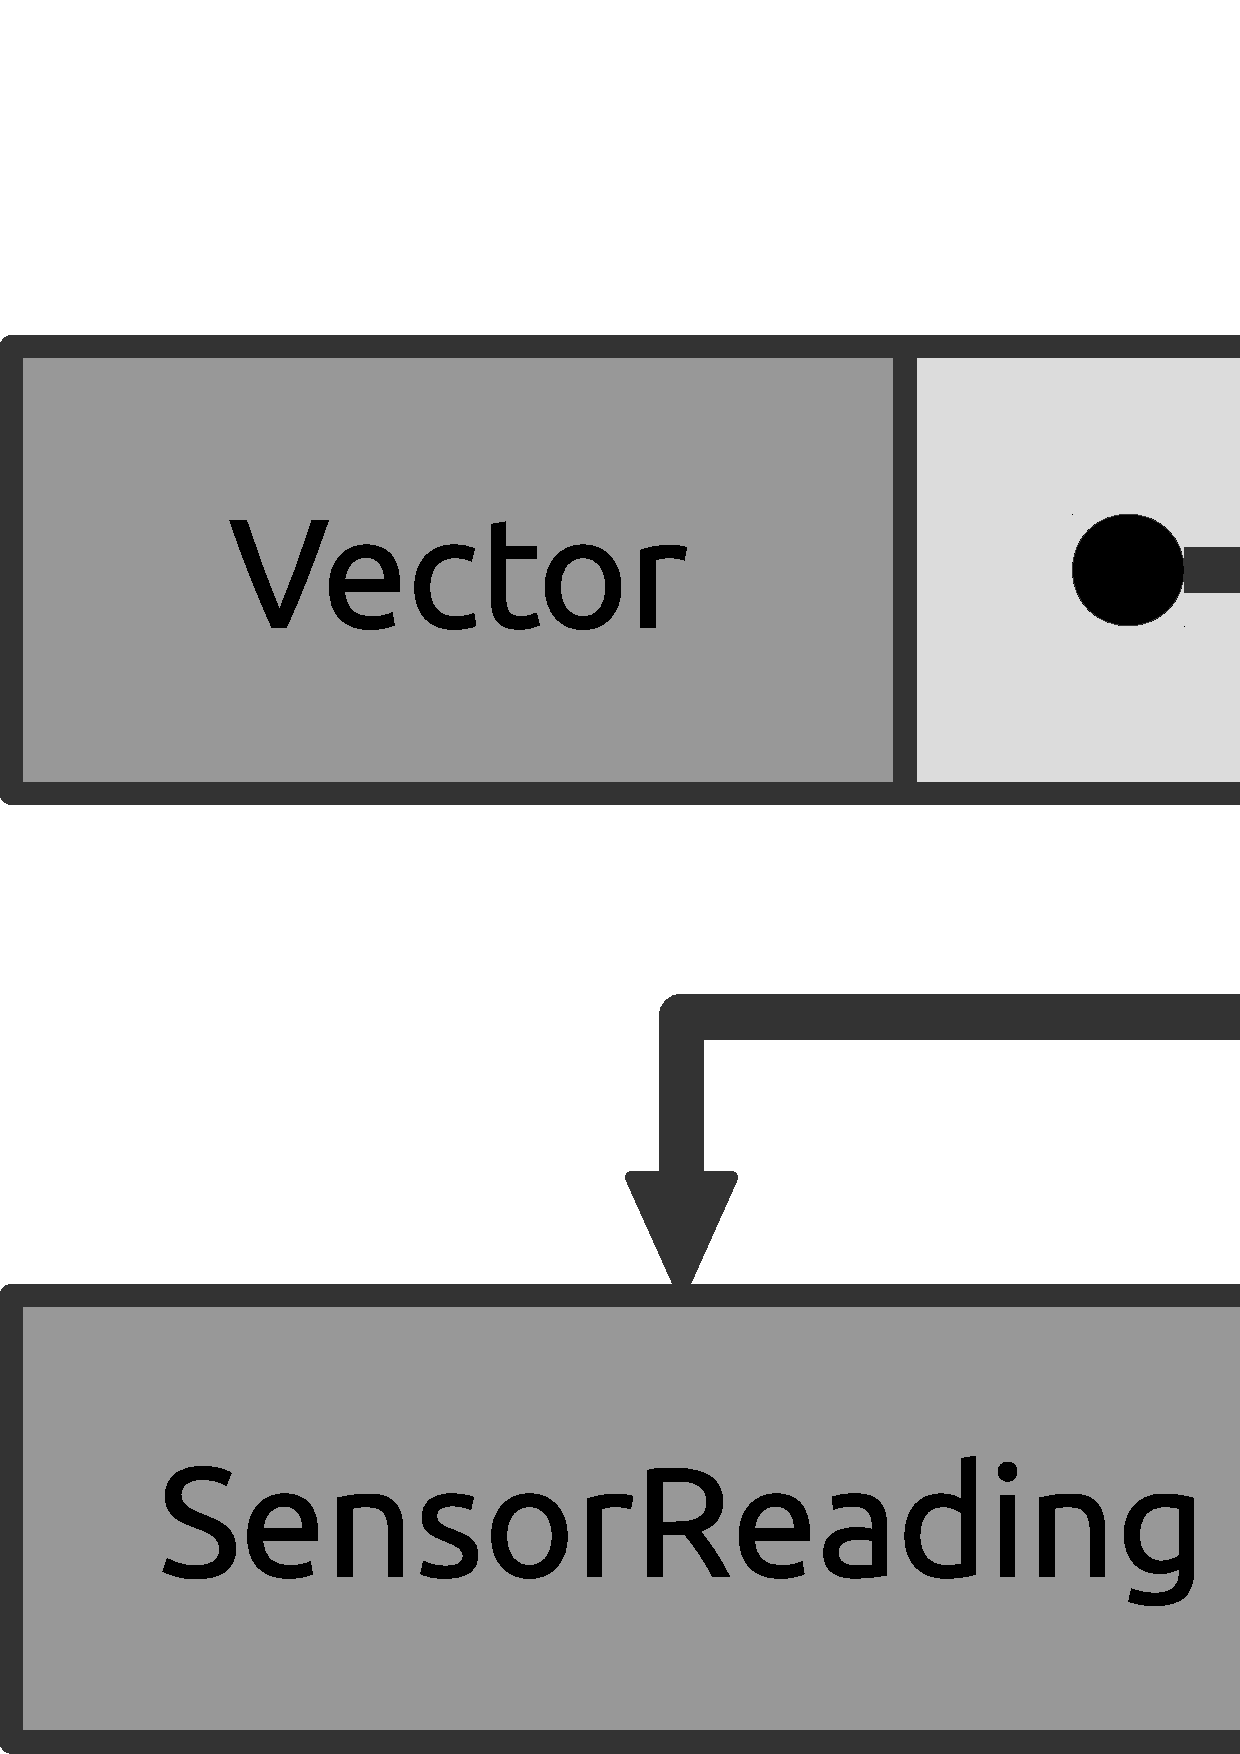
\includegraphics[width=0.95\linewidth]{../graphs/layout/layout2-jvm.pdf}
          \vspace{3mm}
        }

        \vspace{-0.3em}

        Most programmers can immediately give a better layout:

        \separator

        \innerblockplain{
          \vspace{3mm}
          \centering
          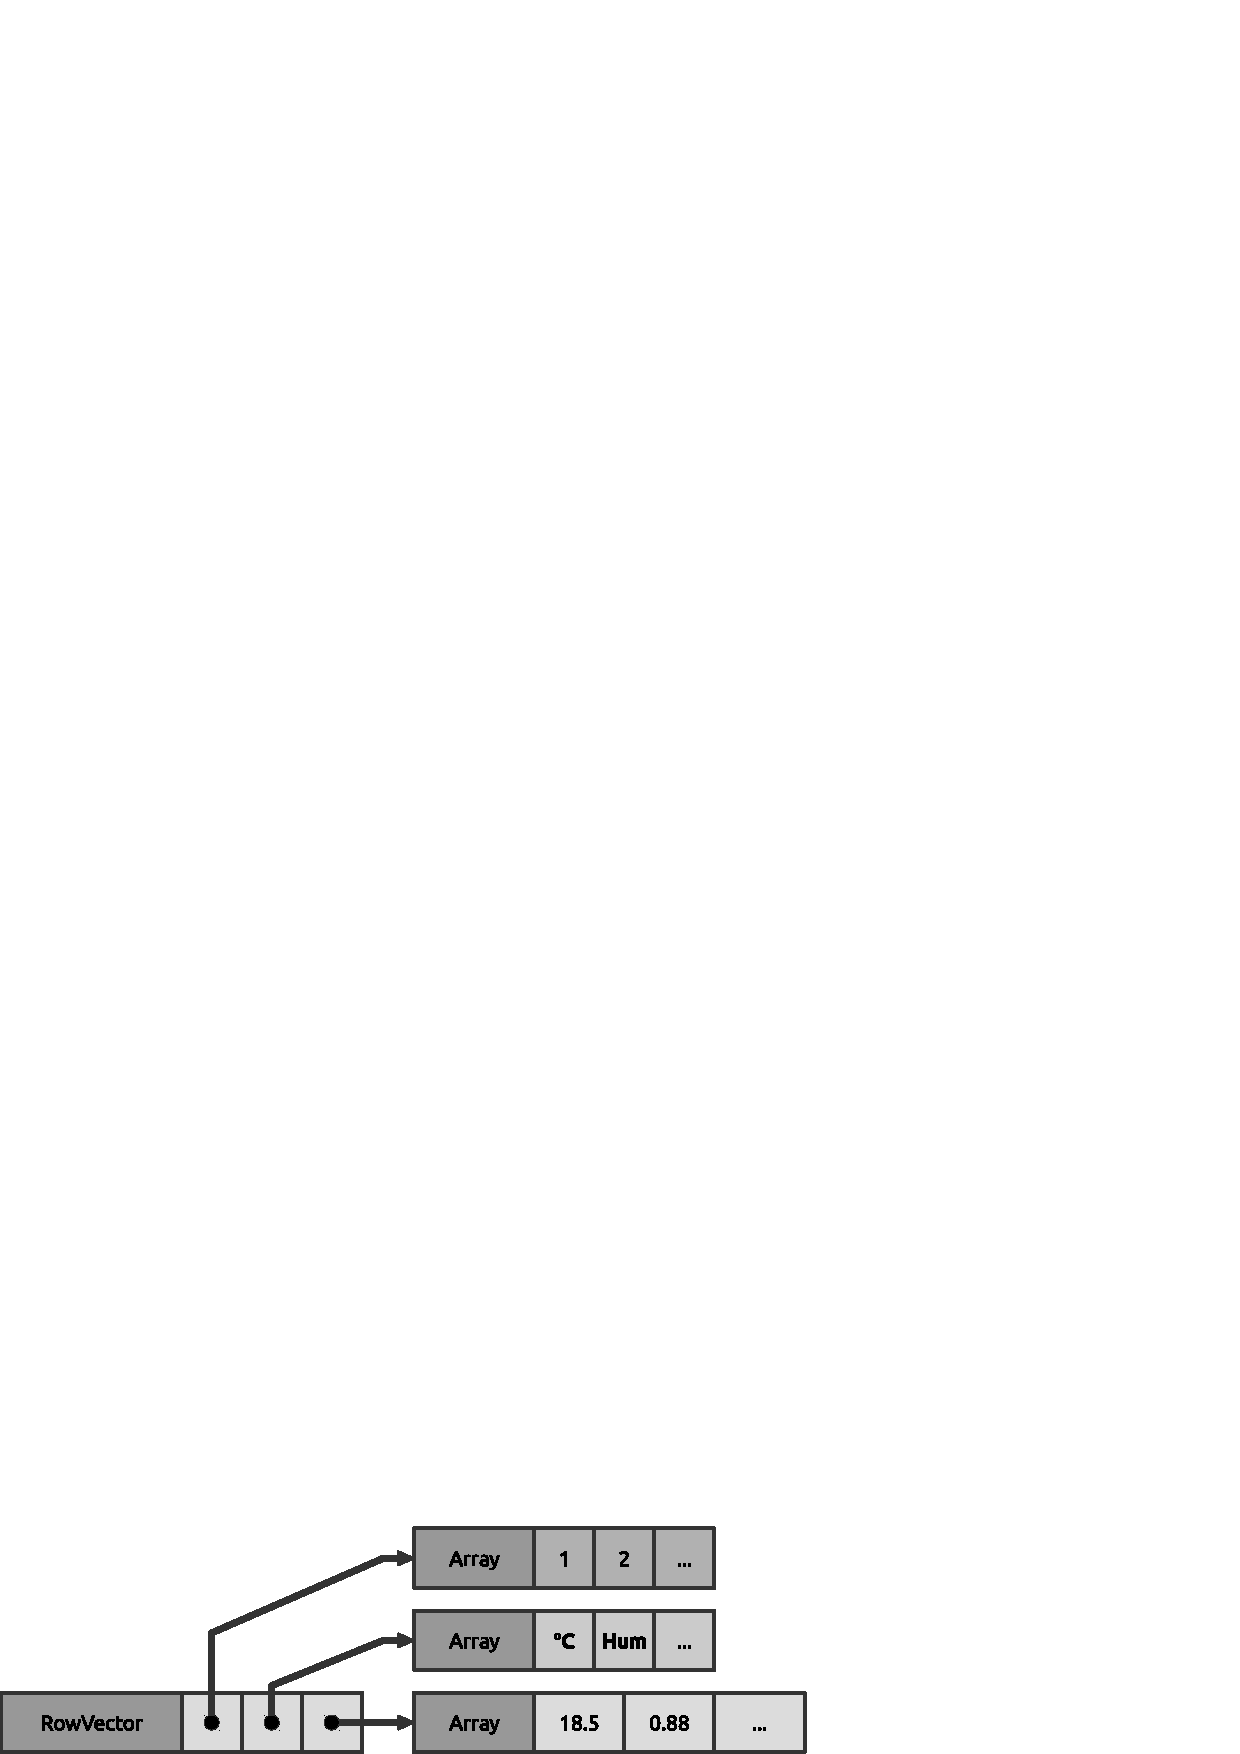
\includegraphics[width=0.95\linewidth]{../graphs/layout/layout2-ideal.pdf}
          \vspace{3mm}
        }

        \vspace{-0.6em}

        But, currently, there is no way for them to modify the data representation, as it is fixed by the compiler.

        \vspace{0.3em}
  }


  \blocknode%
    {\circled{2} Challenges}%
    {\startOfBox

        Optimizing the data representation is difficult:

        \separator

        \ropt{Productivity} Transforming the code by hand is an option, but it is tedious, error prone and harms long-term maintenance.

        \separator

        \ropt{Context dependency} The best layout for a piece of data depends on how it's going to be manipulated and where it's going to be stored. Only the programmer has this information.

        \separator

        \ropt{Open world assumption} New code, which is not aware of the optimized representation, can loaded at any time, thus introducing inconsistencies. Contrarily, most DSLs assume a closed world: only the predefined data structures can be used in the program.

        \separator

        Combined, these three problems make optimizing the data representation very difficult.
  }

  \startsecondcolumn

  \blocknode%
    {\circled{3} Data-centric Optimizations}%
    {\startOfBox

        Data-centric Optimizations overcome the challenges:

        \vspace{-0.2em}
        \separator

        \ropt{Productivity} Our technique extends the Scala compiler to allow trans\-for\-ming the data representation as part of the compilation pipeline, based on \ul{type system information}. Thus, programmers can freely mix and match their data structures.

        \vspace{-0.2em}
        \separator

        \ropt{Context dependency} Since the programmer is in the unique position of deciding the best data layout, we allow them to define it directly in Scala, without any special API:

        \separator

        \codebox{Optimized Data Structure}{
          \code{}{class RowVector(timestamps: Array[Int],  } \\
          \code{................}{sensors: Array[Int]}, \\
          \code{................}{values: Array[Double])}
        }

        \vspace{-0.4em}

        and to instruct the compiler how to use it:

        \separator

        \codebox{Transformation Description Object}{
          \code{}{object RowOpt extends Transformation \{ ... \}  }
        }

        \vspace{-0.6em}

        \separator

        \ropt{Open world assumption} We can enclose a scope where the transformation occurs. Inside, the code uses the optimized representation, while outside, as soon as the value leaks, it is converted to the original encoding:

        \separator

        \codebox{Source Code}{
          \code{}{transform(RowOpt) \{  } \\
          \code{..}{def avgTemp(reads: Vector[...]): Double = ...} \\
          \code{}{\}}
        }
    }
  \vspace{-5mm}

  \blocknode%
    {\circled{4} Composability}%
    {
      \startOfBox
        Transformation scopes can compose (communicate using the optimized data layout) across class boundaries and \ul{even across separate compilation}. If instructed, the compiler can warn when expensive data transformations are necessary:

        \separator

        \codeboxx{Warning}{
          \vspace{0.1em}
          \code{}{warning: When calling method avgTemp, the argument} \\
          \code{}{`data' needs to be converted to the `RowVector'}\\
          \code{}{representation, which may incur some overhead:} \\
          \code{......}{avgTemp(data)} \\
          \code{..............}{\^}
          \vspace{-0.3em}
        }
          \vspace{-0.2em}

      By wrapping the code shown by the warning in the \texttt{transform(RowOpt)\{...\}} scope, the slowdown is avoided, as both the caller and callee will use the optimized layout.
          \vspace{0.2em}
  }
  \vspace{-5mm}

  \blocknode%
    {\circled{5} Benchmarks}%
    {
      \startOfBox
      \innerblockplain{
        \vspace{-12mm}
        \centering
        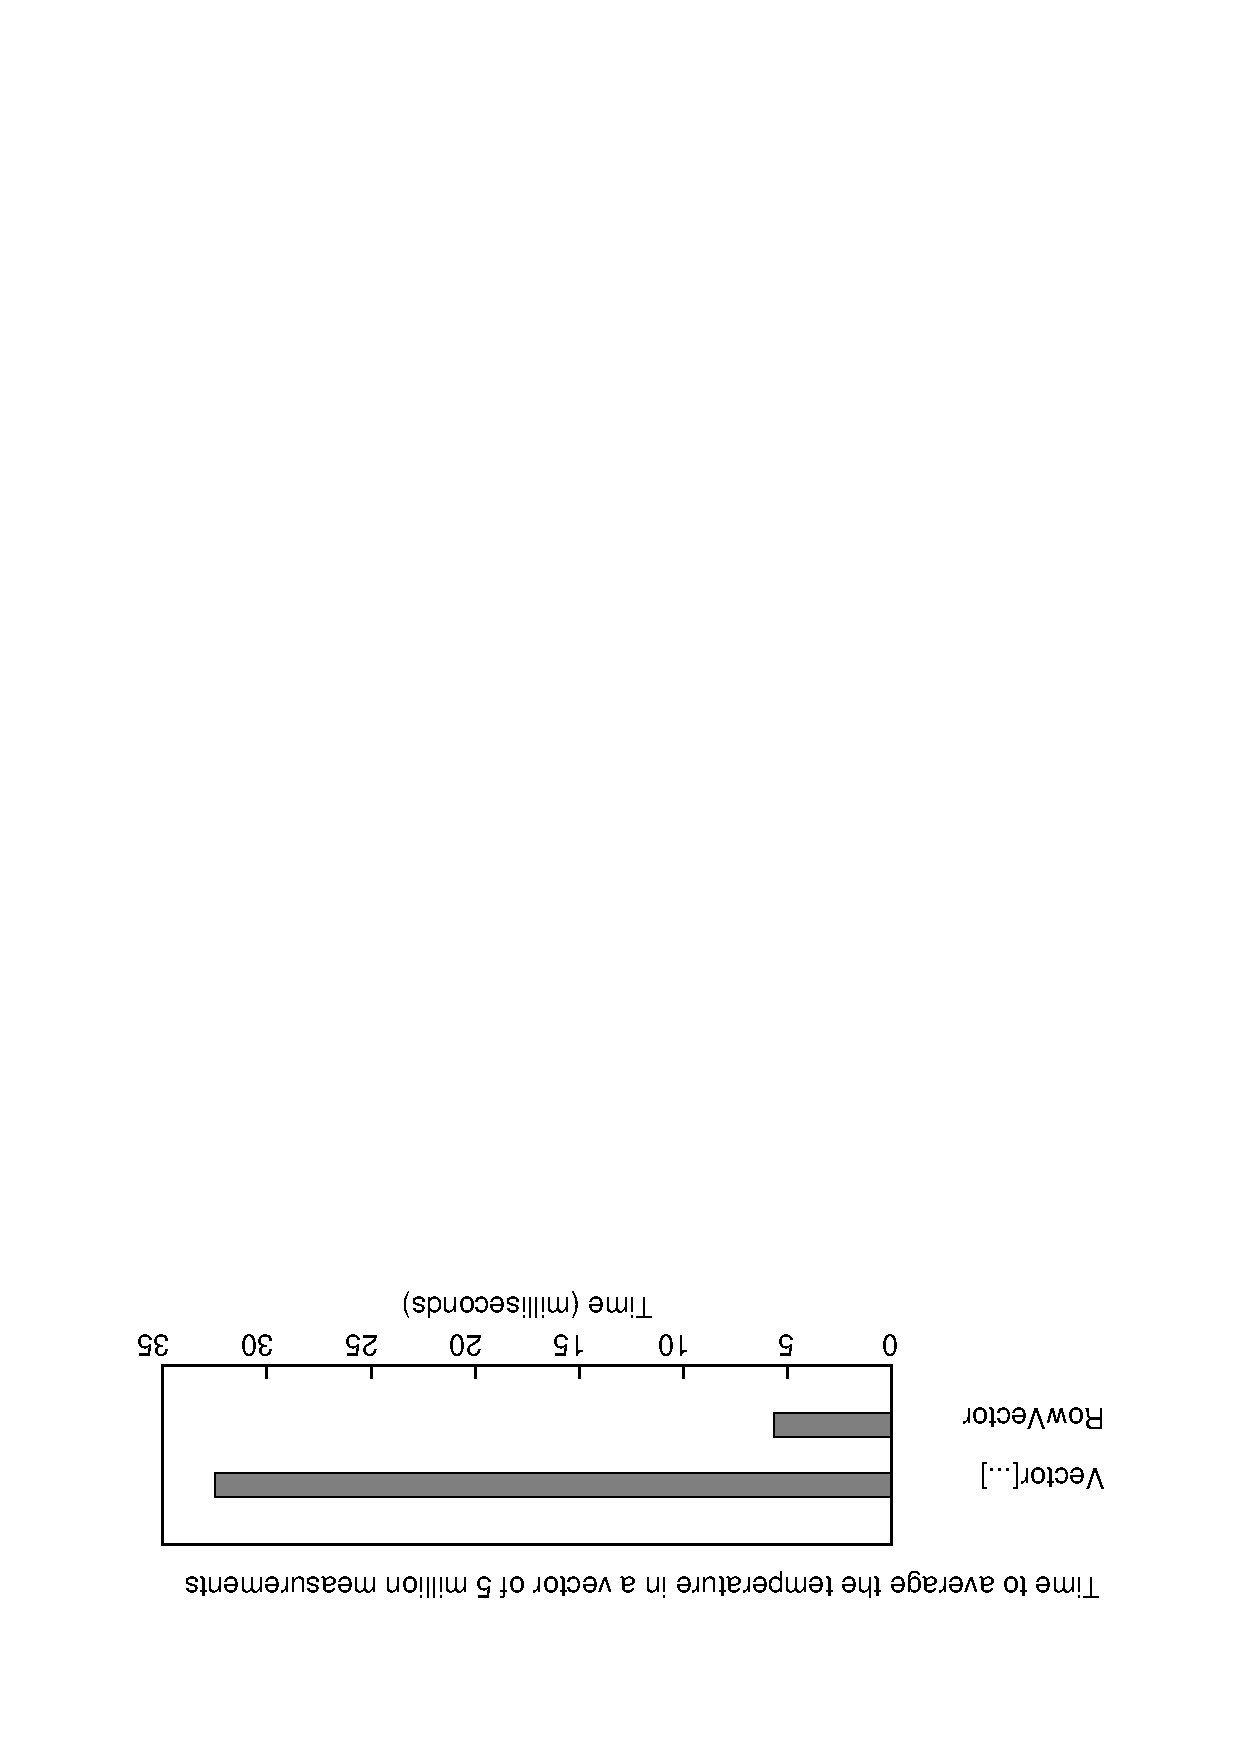
\includegraphics[width=0.99\linewidth,angle=180]{../graphs/speed/speed.pdf}
        \vspace{-7mm}
      }
      \vspace{-0.7em}

      More benchmarks, showing speedups of up to 20x are shown on the project website: \href{http://scala-ildl.org}{\texttt{scala-ildl.org}}

      \vspace{0.2em}
    }

%   \blocknode%
%     {\circled{5} Resources}%
%     {\startOfBox \vspace{-0.3em}
%         %\href{http://scala-miniboxing.org}{\Huge \texttt{\frenchspacing{}scala-miniboxing.org}}
%         %To learn about miniboxing and its implementation as a Scala compiler plugin:
%         \begin{pitemize}
%           \item Official website: \href{http://scala-ildl.org}{\texttt{scala-ildl.org}}
%         \end{pitemize}
%       \vspace{0.1em}
%   }


\end{tikzpicture}


\end{document}




